\documentclass[12pt]{exam}
\usepackage{amsmath}
\usepackage{amssymb}
\usepackage{graphicx}
\usepackage{enumitem}
\usepackage{amsfonts}
\usepackage{amssymb}
\usepackage{ifthen}
\usepackage{geometry}
\noprintanswers

\usepackage{tikz}
\usetikzlibrary{shapes,backgrounds}

\usepackage{framed}

\addtolength{\textheight}{3cm}
\addtolength{\topmargin}{-1cm}
\addtolength{\textwidth}{3cm}
\addtolength{\oddsidemargin}{-1.5cm}
\addtolength{\evensidemargin}{-1.5cm}
\setlength\parindent{0pt}

\newcommand {\DS} [1] {${\displaystyle #1}$}
\newcommand{\vv}{\vspace{.4cm}}

\newcommand{\R}{\mathbb{R}}
\newcommand{\Q}{\mathbb{Q}}
\newcommand{\Z}{\mathbb{Z}}
\newcommand{\N}{\mathbb{N}}

\pagestyle{empty}


%============================================
%137 COLOUR PALETTE
%============================================

\definecolor{137cp1}{RGB}{13, 33, 161}
\definecolor{137cp2}{RGB}{51, 161, 253}
\definecolor{137cp3}{RGB}{255, 67, 101}
\definecolor{137cp4}{RGB}{232, 144, 5}


%============================================
%HYPERLINKS
%============================================

\usepackage{hyperref}
\hypersetup{colorlinks}
\hypersetup{urlcolor=137cp3, linkcolor=137cp1}


%%%%%%%%%%%%%%%%%%%%%%%%%%%%%%%%%%%%%%%%%


\begin{document}

{\large
	\begin{center}
		{\bf MAT 137Y: Calculus with proofs}\\
		{\bf Assignment 3} \\
		{\bf Due on Thursday, November 5 by 11:59pm via Crowdmark}
	\end{center}
}

\vv

\begin{quotation}
{\bf Instructions:}
	\begin{itemize}
		\item	 You will need to submit your solutions electronically via Crowdmark.   \href{https://www.math.toronto.edu/~alfonso/137/PS/137_CM.html}{See MAT137 Crowdmark help page for instructions}.  Make sure you understand how to submit and that you try the system ahead of time.  If you leave it for the last minute and you run into technical problems, you will be late.  There are no extensions for any reason.
		\item You may submit individually or as a team of two students.  See the link above for more details.
		\item  You will need to submit your answer to each question separately.
		\item  This problem set is about derivatives (Unit 3).
	\end{itemize}
\end{quotation}
\vv

\begin{enumerate}

\item The function $g$ has domain $\R$ and is continuous.  Below is the graph of its derivative $g'$.  Sketch the graph of $g$.

	\begin{center}
		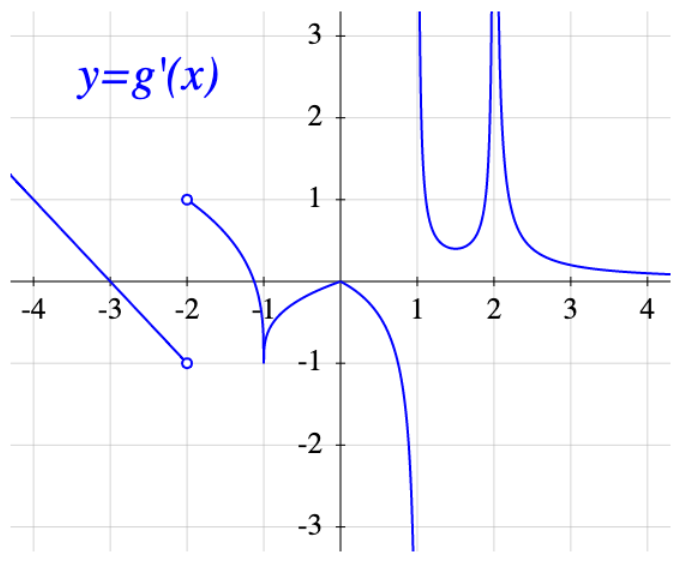
\includegraphics[scale=.5]{A3G1}
	\end{center}

	\emph{Note:} There could be more than one correct answer.

\end{enumerate}

%%%
\newpage

\begin{framed}
{\bf Important!}  We always want you to justify all your answers.  This time, for Q\ref{qu:quotient} and Q\ref{qu:power}, we want you to be particularly careful.  The proofs in those questions contain calculations.   When you are taking those steps, justify everything you do.  Explain explicitly anything you do that is not merely a straightforward algebraic manipulation.  If you are using a hypotheses, say so explicitly.  If you are invoking a theorem, a property, or a previously proven claim, say so explicitly (and make sure you know you are allowed to use it).  We want you to be very conscious of everything you are using and everything you are assuming.
\end{framed}

\begin{enumerate}[resume]

\vv

\item  \label{qu:quotient} 
Let $a \in \R$.  Let $f$ be a function.  Assume $f$ is differentiable at $a$. 

Assume $f$ is never $0$.  Let $g$ be the function defined by the equation \DS{g(x) = \frac{1}{f(x)}}.

Prove that $g$ is differentiable at $a$ and that \DS{g'(a) =  \frac{-f'(a)}{f(a)^2}}. 

Write a proof directly from the definition of derivative, without using any of the differentiation rules.

\vv

\item \label{qu:power}  The power rule says that, for every $c \in \R$:
	$$
		\frac{d}{dx} \left[ x^c \right]  \; = \; c x^{c-1}
	$$
In this problem, we will restrict ourselves only to the domain $x>0$.

In Video 3.7 you learned a proof for a particular case: when $c$ is a positive integer.  You will later (Video 4.10) learn a proof that works for all $c \in \R$ using logarithms, but there are other simple proofs, without using logarithms, that extend to $c \in \Q$.  That is the goal of this problem.
	
You may assume the power rule when $c$ is a positive integer, as well as other results you learned in Unit 3, including the Chain Rule.
	\begin{enumerate}
		\item  Prove the power rule when $c$ is a positive rational.
		
		\emph{Suggestion:}  Assume $c=p/q$ for some positive integers $p$ and $q$.    Define the function $f(x)=x^{p/q}$.  Then this function satisfies
			$$
				f(x)^q = x^p.
			$$
			Use implicit differentiation.
		
		\item  Prove the power rule when $c$ is a negative rational.
		
		\emph{Suggestion:} Look at what you have done so far in this assignment.
	\end{enumerate}

\vv
%%%
\newpage

\item   The function $h$ satisfies the following equation:
	$$ \forall x \in \R, \quad h(xh(x)) = \left[ h(x)\right]^3. $$
In addition, we know:
	\begin{itemize}
		\item The domain of $h$ is $\R$.
		\item $h$ is twice differentiable (meaning that $h$ is differentiable, and $h'$ is also differentiable).
		\item $h(1)=1$.
		\item The graph of $h$ does not have a horizontal tangent line at the point with $x$-coordinate $1$.
	\end{itemize}
	
	Calculate \DS{h''(1)}.
	
	\emph{Hint:} Use implicit differentiation.
	\vv
	\\
	
	\emph{Proof:}\\
	Let $x\in\R.$
	LHS=$h(xh(x))$, RHS=$[h(x)]^3$\\
	Assume the domain of $h$ is $\R$.
	Assume $h(1)=1.$\\
	Assume $h$ is twice differentiable, then $h$ is continuous on $\R$ and $h'$ is continuous on $\R$.\\
	\DS{LHS'}=$h'(xh(x))(xh(x))'$\qquad(Chain Rule)\\
	\DS{LHS'}=$h'(xh(x))(x'h(x)+xh'(x))$\qquad(Product Rule)\\
	\DS{LHS'}=$h'(xh(x))(h(x)+xh'(x))$\qquad(Power Rule) as (1)\\
	\DS{RHS'}=$3[h(x)]^2h'(x)$\qquad(Power and Chain Rule) as (2)\\
	Since $LHS=RHS$, $LHS=RHS \implies LHS'=RHS'$\\
	Evaluating (1) and (2), when $x=1$. \\
	Then,\DS{LHS'}=$h'(1h(1))(h(1)+1h'(1))=h'(1\cdot1)(1+h'(1))=h'(1)(1+h'(1))$\qquad Since($h(1)=1$)\\
	Then,\DS{RHS'}=$3(1)^2h'(1)=3h'(1)$\qquad Since($h(1)=1$)\\
	Suppose $h'(1)=L.$
	Thus,
	\begin{align*}
	    h'(1)(1+h'(1))=3h'(1)\\
	    L(1+L)=3L\\
	    L^2-2L=0\\
	\end{align*}
	This implies $L=0$ or $L=2.$\\
	Since graph of $h$ does not have a horizontal tangent line at the point with x-coordinate 1, this implies $h(1)\neq0$.
	So, $h(1)\neq0\implies h(1)=L=2$\\
	\DS{LHS''}=\DS{(LHS')'}=$(h'(xh(x))(h(x)+xh'(x)))'$\qquad(From (1))\\
	\DS{LHS''}=$h''(xh(x))(xh(x))'(h(x)+xh'(x))+h'(xh(x))(h(x)+xh'(x))'$\qquad(Product and Chain Rule)\\
	\DS{LHS''}=$h''(xh(x))(h(x)+xh'(x))(h(x)+xh'(x))+h'(xh(x))(h(x)+xh'(x))'$\qquad(Product and Power Rule)\\
	\DS{LHS''}=$h''(xh(x))(h(x)+xh'(x))(h(x)+xh'(x))+h'(xh(x))(h'(x)+h'(x)+xh''(x))$\qquad(Sum, Product and Power Rule)\\
	\DS{LHS''}=$h''(xh(x))(h(x)+xh'(x))(h(x)+xh'(x))+h'(xh(x))(2h'(x)+xh''(x))$\qquad as (3)\\
	\DS{RHS''}=\DS{(RHS')'}=$(3[h(x)]^2h'(x))'$\qquad(From (2))\\
	\DS{RHS''}=$3(2h(x)h'(x)h'(x)+[h(x)]^2h''(x))$\qquad(Product and Chain Rule)\\
	\DS{RHS''}=$3[h(x)]^2h''(x)+6h(x)[h'(x)]^2$\qquad as (4)\\
	Since $LHS'=RHS'$, $LHS'=RHS' \implies LHS''=RHS''$\\
	Evaluating (3) and (4), when $x=1$.Then $h(x)=1$ and $h'(x)=2$. \\
	Then, \DS{LHS''}=$h''(1\cdot1)(1+1\cdot2)(1+1\cdot2)+h'(1\cdot1)(2\cdot2+1\cdot h''(1))=9h''(1)+2(4+h''(1))=9h''(1)+8+2h''(1)=11h''(1)+8$\\
	Then, \DS{RHS''}=$3[1]^2h''(1)+6\cdot1[2]^2=3h''(1)+24$\\
	Suppose $h''(1)=M.$
	Thus,
	\begin{align*}
	    11h''(1)+8=3h''(1)+24\\
	    11M+8=3M+24\\
	    8M=16\\
	\end{align*}
	This implies $M=2.$\\
	We have calculated $h''(1)=M=2$ as needed.


\end{enumerate}
\end{document}


